% Options for packages loaded elsewhere
\PassOptionsToPackage{unicode}{hyperref}
\PassOptionsToPackage{hyphens}{url}
%
\documentclass[
]{article}
\usepackage{amsmath,amssymb}
\usepackage{lmodern}
\usepackage{ifxetex,ifluatex}
\ifnum 0\ifxetex 1\fi\ifluatex 1\fi=0 % if pdftex
  \usepackage[T1]{fontenc}
  \usepackage[utf8]{inputenc}
  \usepackage{textcomp} % provide euro and other symbols
\else % if luatex or xetex
  \usepackage{unicode-math}
  \defaultfontfeatures{Scale=MatchLowercase}
  \defaultfontfeatures[\rmfamily]{Ligatures=TeX,Scale=1}
\fi
% Use upquote if available, for straight quotes in verbatim environments
\IfFileExists{upquote.sty}{\usepackage{upquote}}{}
\IfFileExists{microtype.sty}{% use microtype if available
  \usepackage[]{microtype}
  \UseMicrotypeSet[protrusion]{basicmath} % disable protrusion for tt fonts
}{}
\makeatletter
\@ifundefined{KOMAClassName}{% if non-KOMA class
  \IfFileExists{parskip.sty}{%
    \usepackage{parskip}
  }{% else
    \setlength{\parindent}{0pt}
    \setlength{\parskip}{6pt plus 2pt minus 1pt}}
}{% if KOMA class
  \KOMAoptions{parskip=half}}
\makeatother
\usepackage{xcolor}
\IfFileExists{xurl.sty}{\usepackage{xurl}}{} % add URL line breaks if available
\IfFileExists{bookmark.sty}{\usepackage{bookmark}}{\usepackage{hyperref}}
\hypersetup{
  pdftitle={The power of RNotebook + GitHub + Overleaf},
  hidelinks,
  pdfcreator={LaTeX via pandoc}}
\urlstyle{same} % disable monospaced font for URLs
\usepackage[margin=1in]{geometry}
\usepackage{color}
\usepackage{fancyvrb}
\newcommand{\VerbBar}{|}
\newcommand{\VERB}{\Verb[commandchars=\\\{\}]}
\DefineVerbatimEnvironment{Highlighting}{Verbatim}{commandchars=\\\{\}}
% Add ',fontsize=\small' for more characters per line
\usepackage{framed}
\definecolor{shadecolor}{RGB}{248,248,248}
\newenvironment{Shaded}{\begin{snugshade}}{\end{snugshade}}
\newcommand{\AlertTok}[1]{\textcolor[rgb]{0.94,0.16,0.16}{#1}}
\newcommand{\AnnotationTok}[1]{\textcolor[rgb]{0.56,0.35,0.01}{\textbf{\textit{#1}}}}
\newcommand{\AttributeTok}[1]{\textcolor[rgb]{0.77,0.63,0.00}{#1}}
\newcommand{\BaseNTok}[1]{\textcolor[rgb]{0.00,0.00,0.81}{#1}}
\newcommand{\BuiltInTok}[1]{#1}
\newcommand{\CharTok}[1]{\textcolor[rgb]{0.31,0.60,0.02}{#1}}
\newcommand{\CommentTok}[1]{\textcolor[rgb]{0.56,0.35,0.01}{\textit{#1}}}
\newcommand{\CommentVarTok}[1]{\textcolor[rgb]{0.56,0.35,0.01}{\textbf{\textit{#1}}}}
\newcommand{\ConstantTok}[1]{\textcolor[rgb]{0.00,0.00,0.00}{#1}}
\newcommand{\ControlFlowTok}[1]{\textcolor[rgb]{0.13,0.29,0.53}{\textbf{#1}}}
\newcommand{\DataTypeTok}[1]{\textcolor[rgb]{0.13,0.29,0.53}{#1}}
\newcommand{\DecValTok}[1]{\textcolor[rgb]{0.00,0.00,0.81}{#1}}
\newcommand{\DocumentationTok}[1]{\textcolor[rgb]{0.56,0.35,0.01}{\textbf{\textit{#1}}}}
\newcommand{\ErrorTok}[1]{\textcolor[rgb]{0.64,0.00,0.00}{\textbf{#1}}}
\newcommand{\ExtensionTok}[1]{#1}
\newcommand{\FloatTok}[1]{\textcolor[rgb]{0.00,0.00,0.81}{#1}}
\newcommand{\FunctionTok}[1]{\textcolor[rgb]{0.00,0.00,0.00}{#1}}
\newcommand{\ImportTok}[1]{#1}
\newcommand{\InformationTok}[1]{\textcolor[rgb]{0.56,0.35,0.01}{\textbf{\textit{#1}}}}
\newcommand{\KeywordTok}[1]{\textcolor[rgb]{0.13,0.29,0.53}{\textbf{#1}}}
\newcommand{\NormalTok}[1]{#1}
\newcommand{\OperatorTok}[1]{\textcolor[rgb]{0.81,0.36,0.00}{\textbf{#1}}}
\newcommand{\OtherTok}[1]{\textcolor[rgb]{0.56,0.35,0.01}{#1}}
\newcommand{\PreprocessorTok}[1]{\textcolor[rgb]{0.56,0.35,0.01}{\textit{#1}}}
\newcommand{\RegionMarkerTok}[1]{#1}
\newcommand{\SpecialCharTok}[1]{\textcolor[rgb]{0.00,0.00,0.00}{#1}}
\newcommand{\SpecialStringTok}[1]{\textcolor[rgb]{0.31,0.60,0.02}{#1}}
\newcommand{\StringTok}[1]{\textcolor[rgb]{0.31,0.60,0.02}{#1}}
\newcommand{\VariableTok}[1]{\textcolor[rgb]{0.00,0.00,0.00}{#1}}
\newcommand{\VerbatimStringTok}[1]{\textcolor[rgb]{0.31,0.60,0.02}{#1}}
\newcommand{\WarningTok}[1]{\textcolor[rgb]{0.56,0.35,0.01}{\textbf{\textit{#1}}}}
\usepackage{graphicx}
\makeatletter
\def\maxwidth{\ifdim\Gin@nat@width>\linewidth\linewidth\else\Gin@nat@width\fi}
\def\maxheight{\ifdim\Gin@nat@height>\textheight\textheight\else\Gin@nat@height\fi}
\makeatother
% Scale images if necessary, so that they will not overflow the page
% margins by default, and it is still possible to overwrite the defaults
% using explicit options in \includegraphics[width, height, ...]{}
\setkeys{Gin}{width=\maxwidth,height=\maxheight,keepaspectratio}
% Set default figure placement to htbp
\makeatletter
\def\fps@figure{htbp}
\makeatother
\setlength{\emergencystretch}{3em} % prevent overfull lines
\providecommand{\tightlist}{%
  \setlength{\itemsep}{0pt}\setlength{\parskip}{0pt}}
\setcounter{secnumdepth}{-\maxdimen} % remove section numbering
\ifluatex
  \usepackage{selnolig}  % disable illegal ligatures
\fi

\title{The power of RNotebook + GitHub + Overleaf}
\author{}
\date{\vspace{-2.5em}}

\begin{document}
\maketitle

This is an \href{http://rmarkdown.rstudio.com}{R Markdown} Notebook.
When you execute code within the notebook, the results appear beneath
the code.

These code blocks are where I keep all of my notes \& working thoughts
on figure generation and analyses. When you ``Knit'' the R Notebook, it
converts this markdown file to other document formats, such as PDF or
HTML. This format is useful \emph{in place of} creating a powerpoint of
your figures because you can integrate your code and annotations all in
one! And send to others as a single document. However, one downside is -
if your code takes awhile to process (large dataset/many iterations), it
will take that much longer to knit. This can be frustrating when
producing a final product. I would recommend working with the products
of your analyses by importing files created in other scripts, instead of
trying to generate everything in the Rmd. When importing the datasets
from other scripts/locations, just make sure to document VERY well what
script generated it \& where the data live.

\begin{center}\rule{0.5\linewidth}{0.5pt}\end{center}

This first chunk is the setup chunk. Currently, this will not appear in
your knitted document because of ``include=FALSE'' (i.e.~do NOT include
this chunk in the output pdf/html). You can always remove the
``include=FALSE'' argument from the brackets to make more transparent
what was required for your notebook (i.e.~include in the output pdf all
packages used and information to set up your .Rmd.

\textbf{Here we do 4 things in the set up brackets:}

\begin{enumerate}
\def\labelenumi{\arabic{enumi}.}
\tightlist
\item
  Designate this is R code (you can run other languages)
\item
  Load the built-in cars dataset
\item
  indicate global options are being set
\item
  indicate the include=FALSE, do NOT include this chunk in the knit
  document
\end{enumerate}

\textbf{Then, set knitr options:} \emph{Specifically, we tell knitr how
to create figures and where to write them out (i.e.~our repository!)}

\textbf{Then, we load any necessary packages used in the .Rmd}

Try executing this chunk by clicking the \emph{Run} button within the
chunk or by placing your cursor inside it and pressing
\emph{Ctrl+Shift+Enter}.

Above, I changed the font (bold, italicized), but there are built-in
ways to organize your document. Different headings, as seen below, are
useful for guiding readers through a more ``outlined'' document.

\hypertarget{yay-for-plots}{%
\section{Yay for Plots!}\label{yay-for-plots}}

\hypertarget{using-built-in-r-data-base-r}{%
\subsection{Using built-in R data \& Base
R}\label{using-built-in-r-data-base-r}}

\hypertarget{ooooooh-aaaaaahhhh-in-line-code}{%
\subsubsection{Ooooooh aaaaaahhhh, in-line
code}\label{ooooooh-aaaaaahhhh-in-line-code}}

There are 50 records in the cars dataset.

\begin{Shaded}
\begin{Highlighting}[]
\CommentTok{\#plot speed over distance}
\FunctionTok{plot}\NormalTok{(cars}\SpecialCharTok{$}\NormalTok{speed,cars}\SpecialCharTok{$}\NormalTok{dist)}
\end{Highlighting}
\end{Shaded}

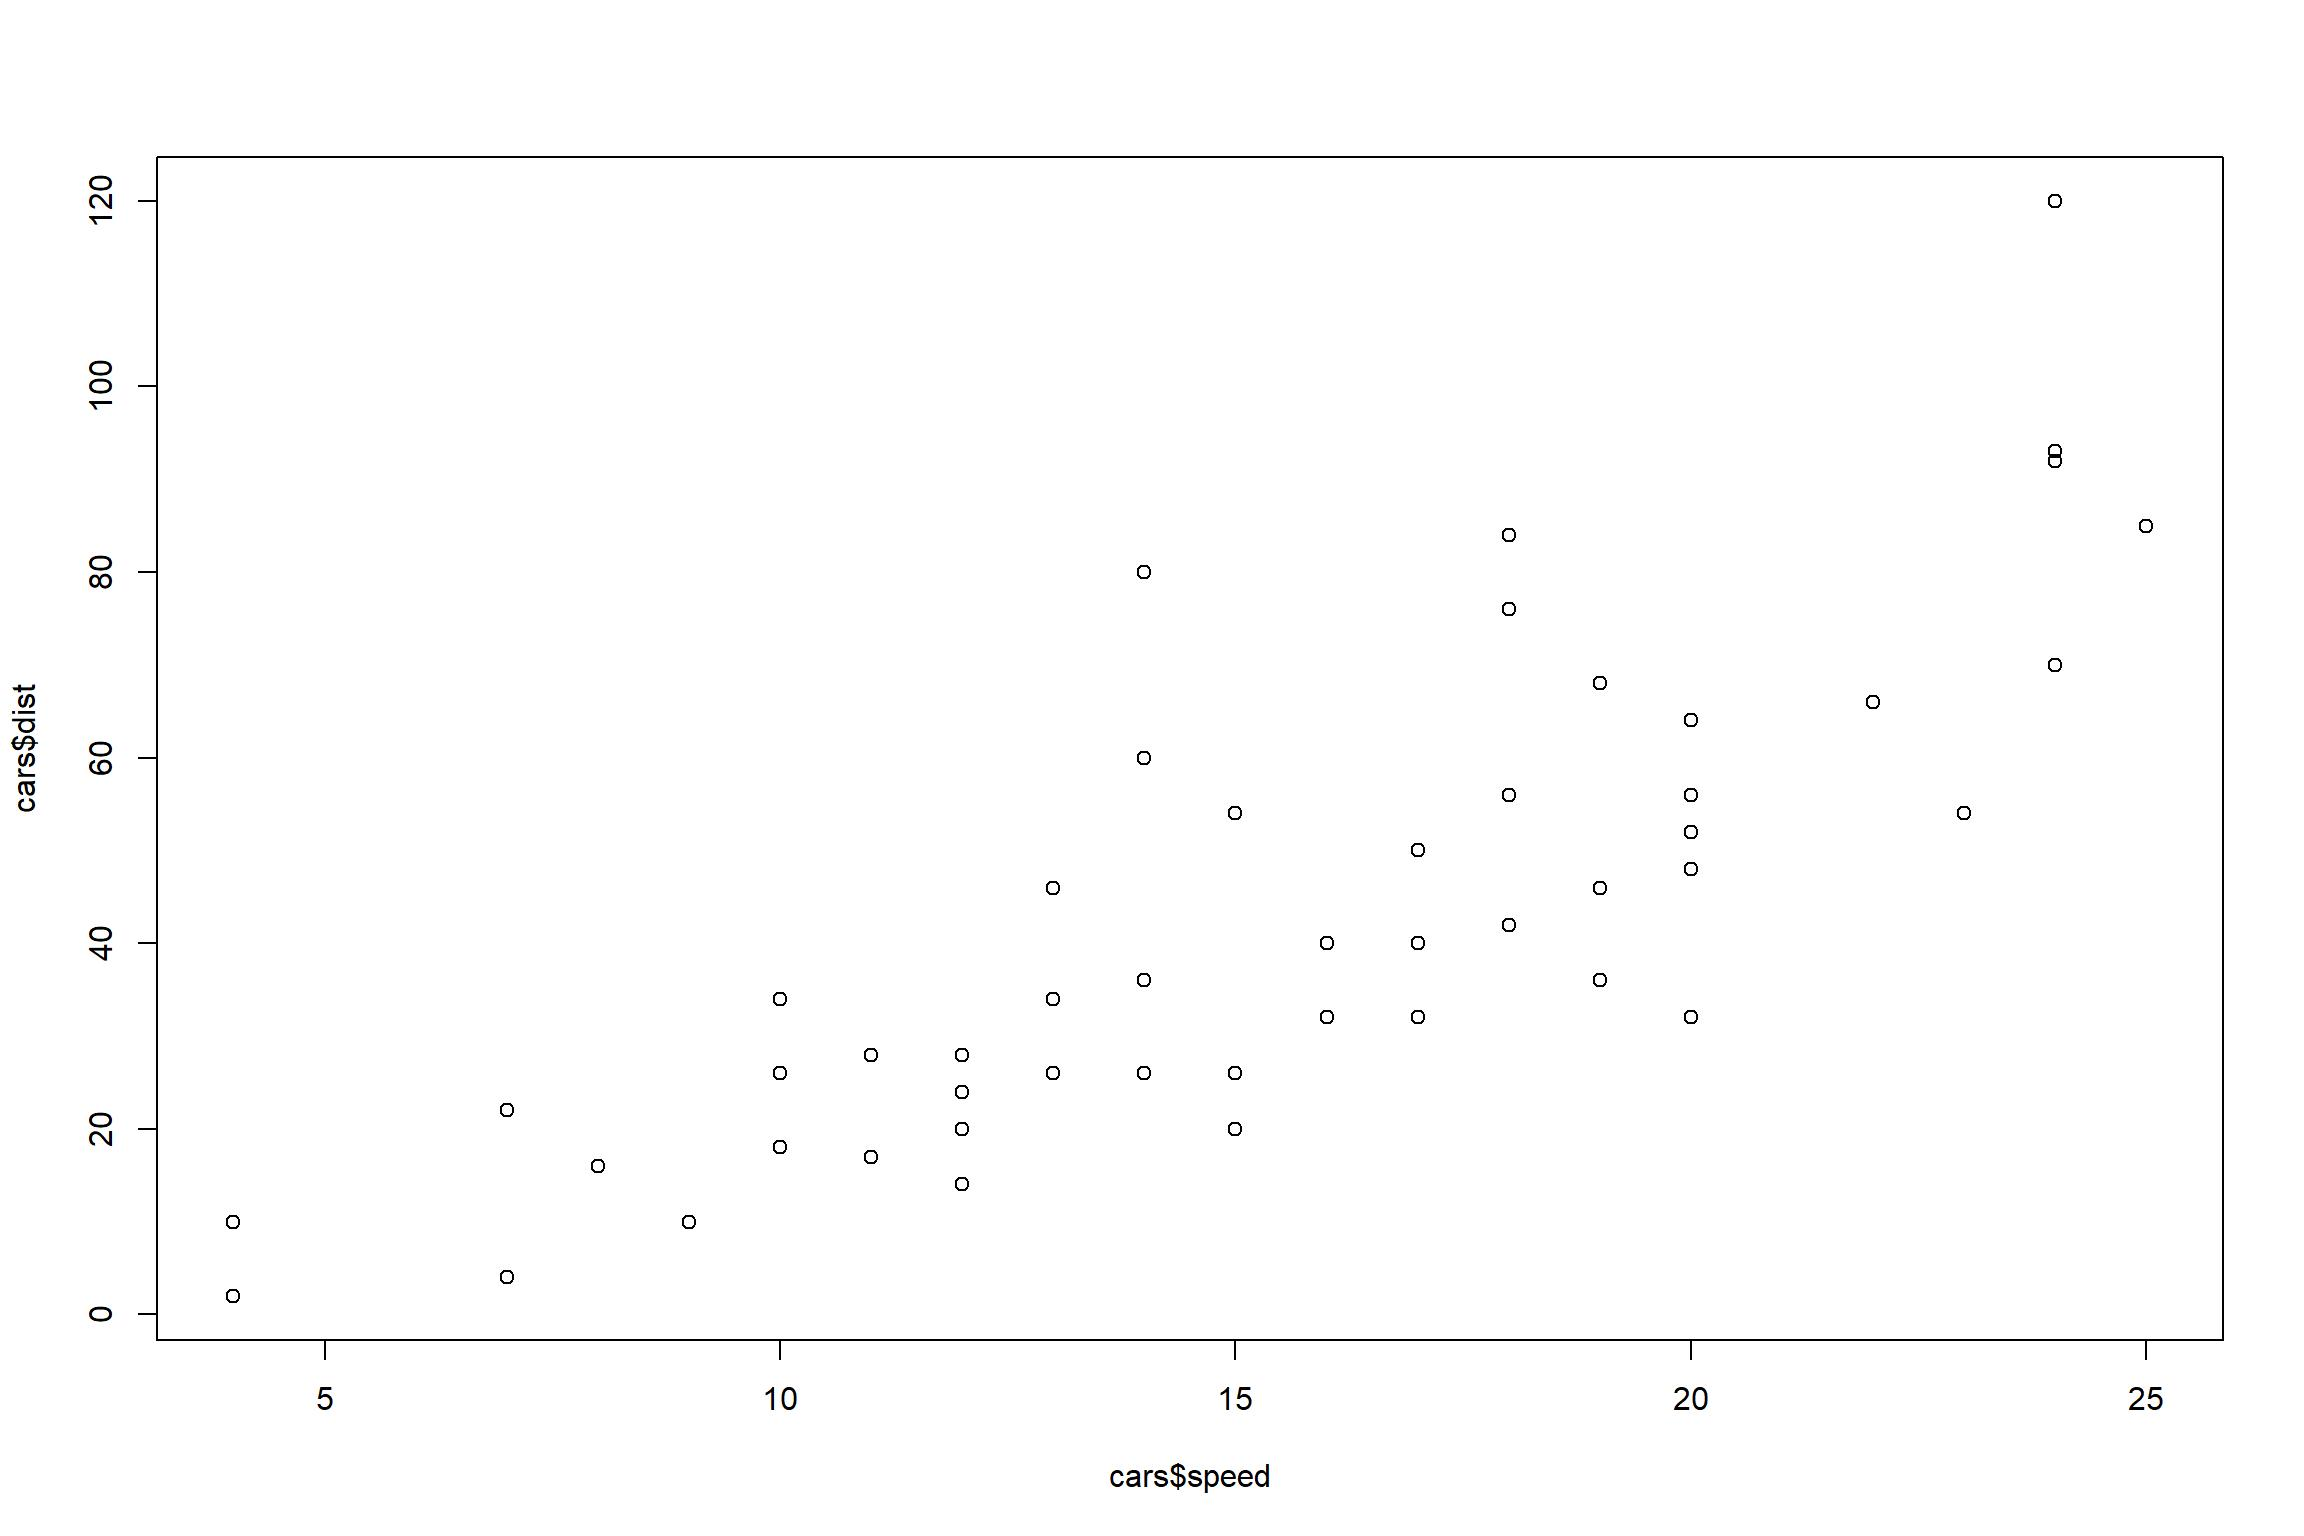
\includegraphics{figures/Cars-speed_dist-1.jpeg}

\begin{Shaded}
\begin{Highlighting}[]
\CommentTok{\#same plot, but improved! color, aces labels, symbol type specification, and title}
\FunctionTok{plot}\NormalTok{(cars}\SpecialCharTok{$}\NormalTok{speed,cars}\SpecialCharTok{$}\NormalTok{dist,}\AttributeTok{col=}\StringTok{"blue"}\NormalTok{,}\AttributeTok{xlab=}\StringTok{"Speed"}\NormalTok{,}\AttributeTok{ylab=}\StringTok{"Distance"}\NormalTok{,}\AttributeTok{pch=}\DecValTok{16}\NormalTok{,}\AttributeTok{main=}\StringTok{"Cars Speed \& Distance : n=50"}\NormalTok{)}
\end{Highlighting}
\end{Shaded}

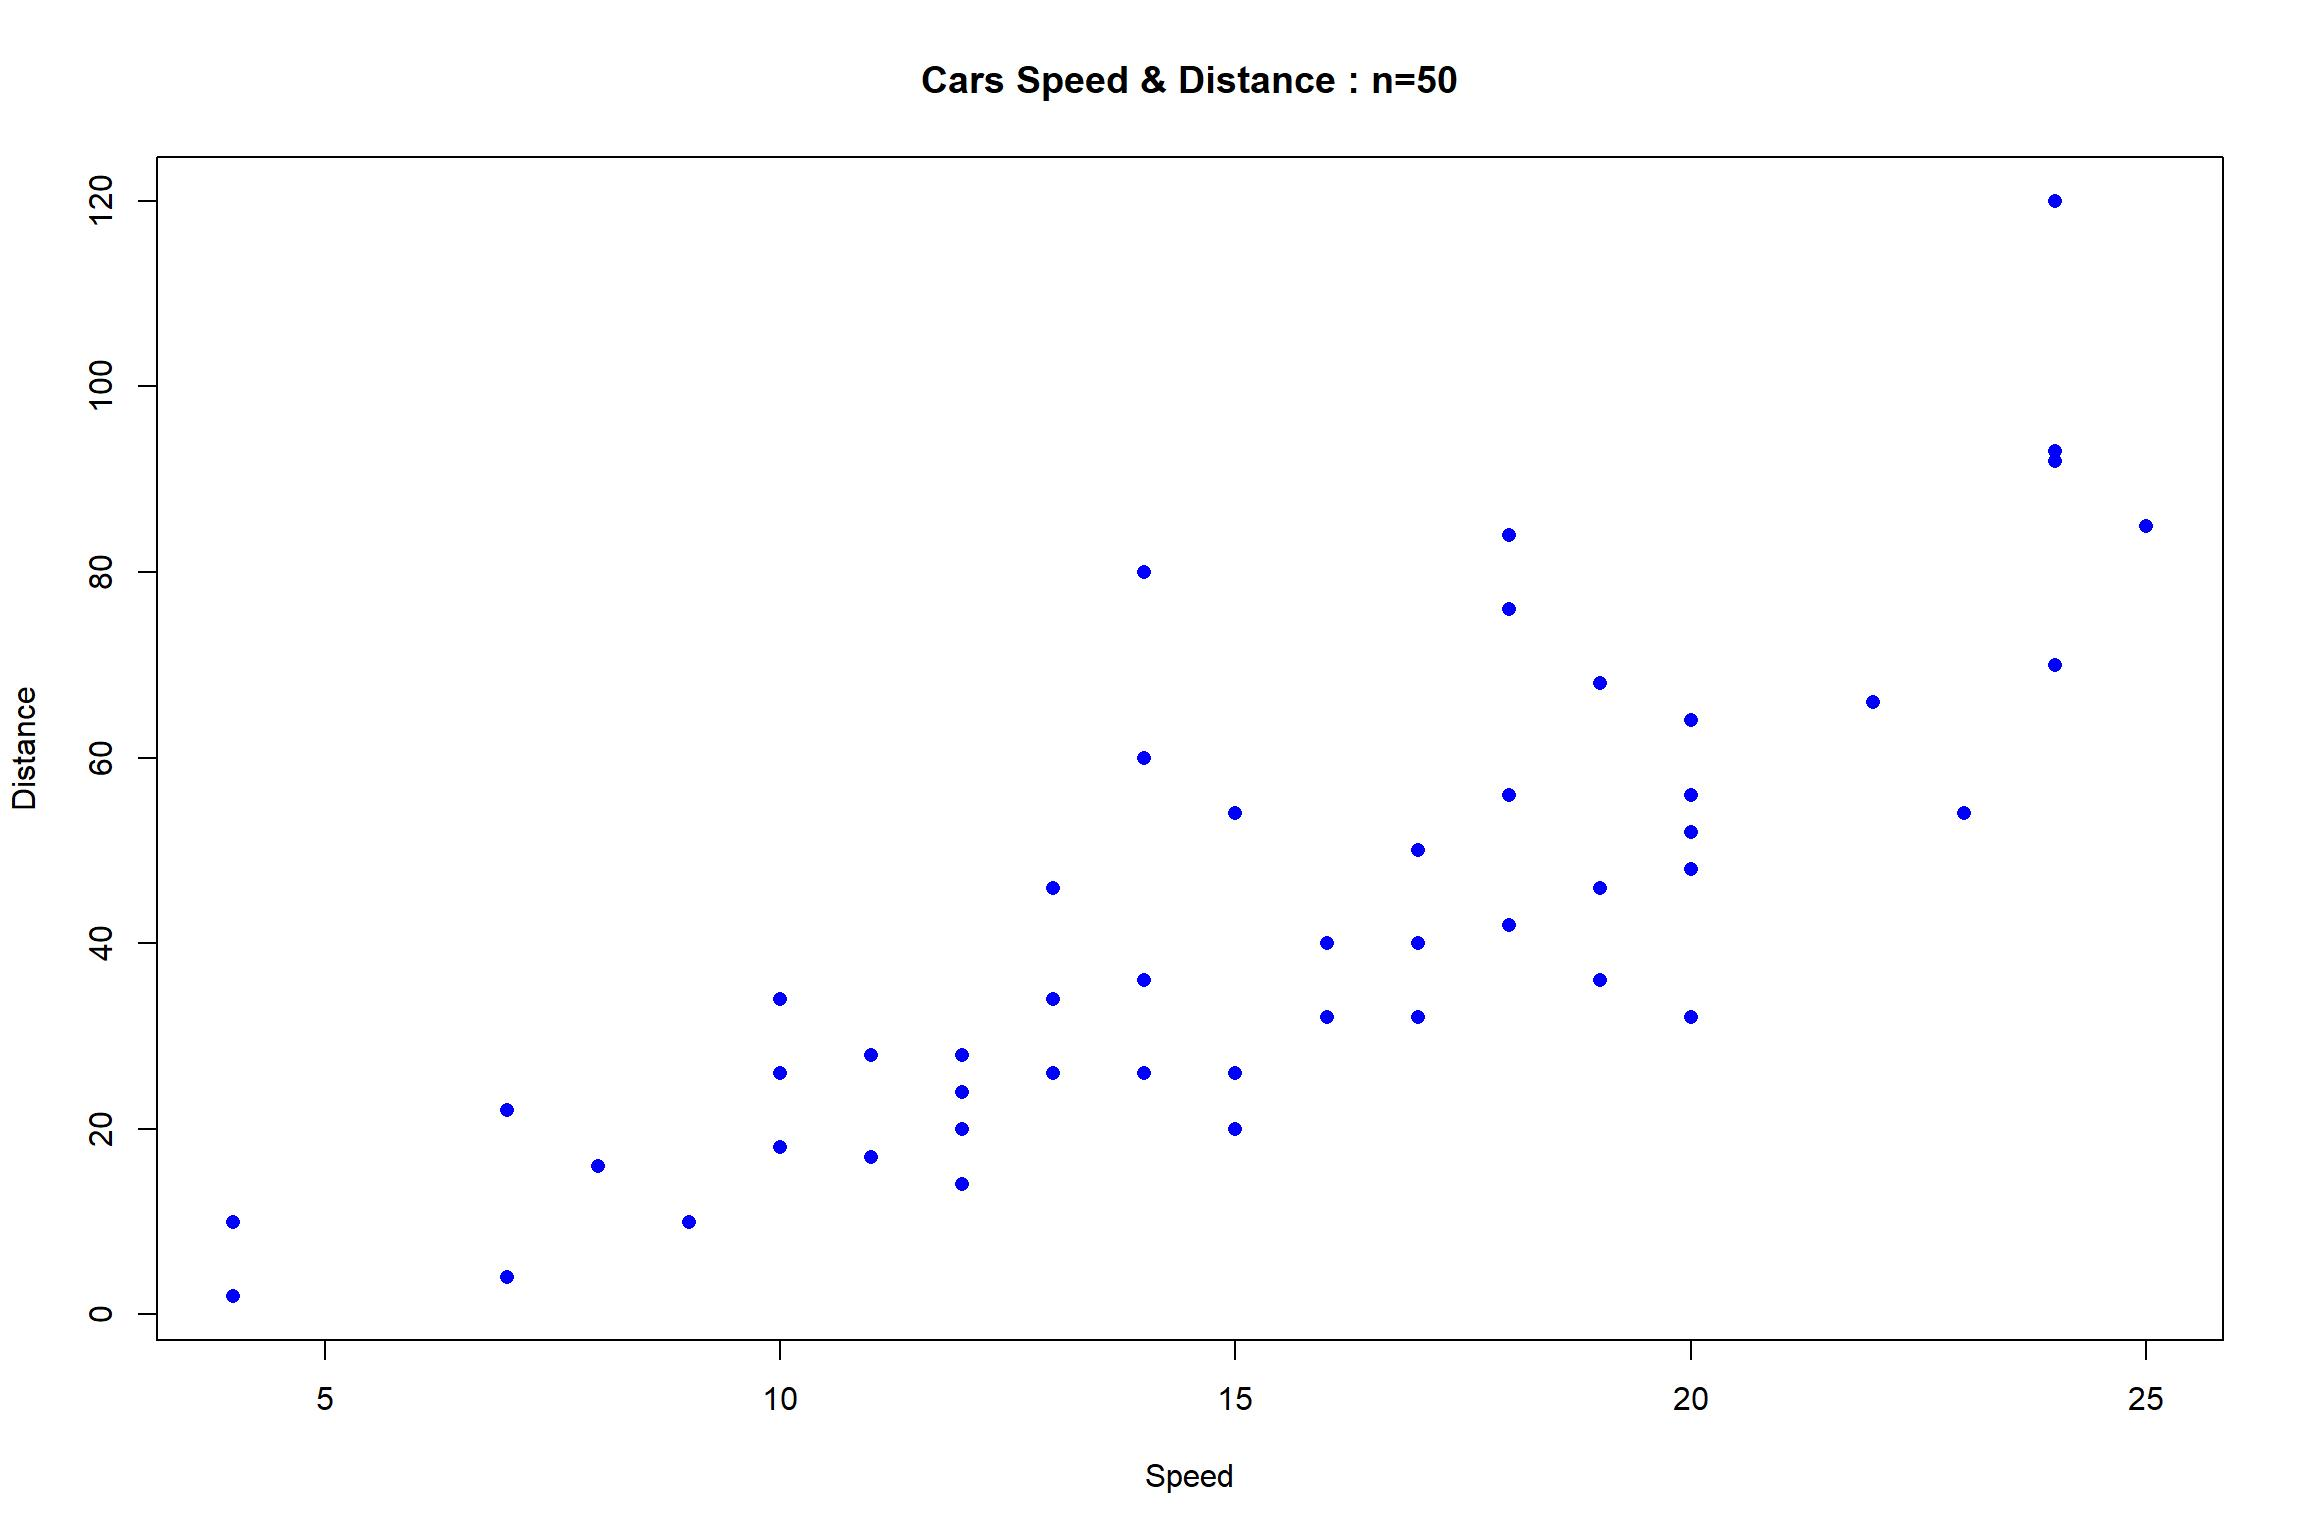
\includegraphics{figures/Cars-speed_dist-2.jpeg}

\begin{Shaded}
\begin{Highlighting}[]
\CommentTok{\#we can write out any dataframe as csv }
\FunctionTok{write.csv}\NormalTok{(cars\_df,}\StringTok{"cars.csv"}\NormalTok{)}
\end{Highlighting}
\end{Shaded}

\hypertarget{plot-midwest-data}{%
\section{Plot Midwest Data}\label{plot-midwest-data}}

\hypertarget{use-ggplot}{%
\subsection{Use ggplot}\label{use-ggplot}}

\hypertarget{learn-about-plot-strucure-themes}{%
\subsubsection{Learn about plot strucure \&
themes!}\label{learn-about-plot-strucure-themes}}

Plots examples below and more from this website:

\url{http://r-statistics.co/Top50-Ggplot2-Visualizations-MasterList-R-Code.html\#Bubble\%20Plot}

\begin{Shaded}
\begin{Highlighting}[]
\CommentTok{\#specify midwest data from ggplot2 (may be redundant with loading it in the setup brackets?)}
\FunctionTok{data}\NormalTok{(}\StringTok{"midwest"}\NormalTok{, }\AttributeTok{package =} \StringTok{"ggplot2"}\NormalTok{)}

\CommentTok{\#specify as dataframe, this is a step I generally do, but is not always necessary}
\NormalTok{midwest\_df}\OtherTok{\textless{}{-}}\FunctionTok{as.data.frame}\NormalTok{(midwest)}

\CommentTok{\# Creating a scatterplot w/ ggplot}
\NormalTok{gg }\OtherTok{\textless{}{-}} \FunctionTok{ggplot}\NormalTok{(midwest, }\FunctionTok{aes}\NormalTok{(}\AttributeTok{x=}\NormalTok{area, }\AttributeTok{y=}\NormalTok{poptotal)) }\SpecialCharTok{+} \CommentTok{\#plot with specifying data as x,y }
  \FunctionTok{geom\_point}\NormalTok{(}\FunctionTok{aes}\NormalTok{(}\AttributeTok{col=}\NormalTok{state, }\AttributeTok{size=}\NormalTok{popdensity)) }\SpecialCharTok{+} \CommentTok{\#color the scatterplot by state and size the dots by popdensity}
  \FunctionTok{geom\_smooth}\NormalTok{(}\AttributeTok{method=}\StringTok{"loess"}\NormalTok{, }\AttributeTok{se=}\NormalTok{F) }\SpecialCharTok{+} \CommentTok{\#loess = "smooth local regression"}
  \FunctionTok{xlim}\NormalTok{(}\FunctionTok{c}\NormalTok{(}\DecValTok{0}\NormalTok{, }\FloatTok{0.1}\NormalTok{)) }\SpecialCharTok{+} \CommentTok{\#x{-}zaxis limits}
  \FunctionTok{ylim}\NormalTok{(}\FunctionTok{c}\NormalTok{(}\DecValTok{0}\NormalTok{, }\DecValTok{500000}\NormalTok{)) }\SpecialCharTok{+} \CommentTok{\#y{-}axis limits}
  \FunctionTok{labs}\NormalTok{(}\AttributeTok{subtitle=}\StringTok{"Area Vs Population"}\NormalTok{,  }\CommentTok{\#specify all labels}
       \AttributeTok{y=}\StringTok{"Population"}\NormalTok{, }
       \AttributeTok{x=}\StringTok{"Area"}\NormalTok{, }
       \AttributeTok{title=}\StringTok{"Scatterplot"}\NormalTok{, }
       \AttributeTok{caption =} \StringTok{"Source: midwest"}\NormalTok{)}

\CommentTok{\#here we can plots or design elements together to create a new plot}
\CommentTok{\#it doesn\textquotesingle{}t plot the plot, until calling "plot" (below)}
\NormalTok{gg\_themed}\OtherTok{\textless{}{-}}\NormalTok{ gg }\SpecialCharTok{+}  \FunctionTok{theme\_tufte}\NormalTok{() }

\FunctionTok{plot}\NormalTok{(gg)}
\end{Highlighting}
\end{Shaded}

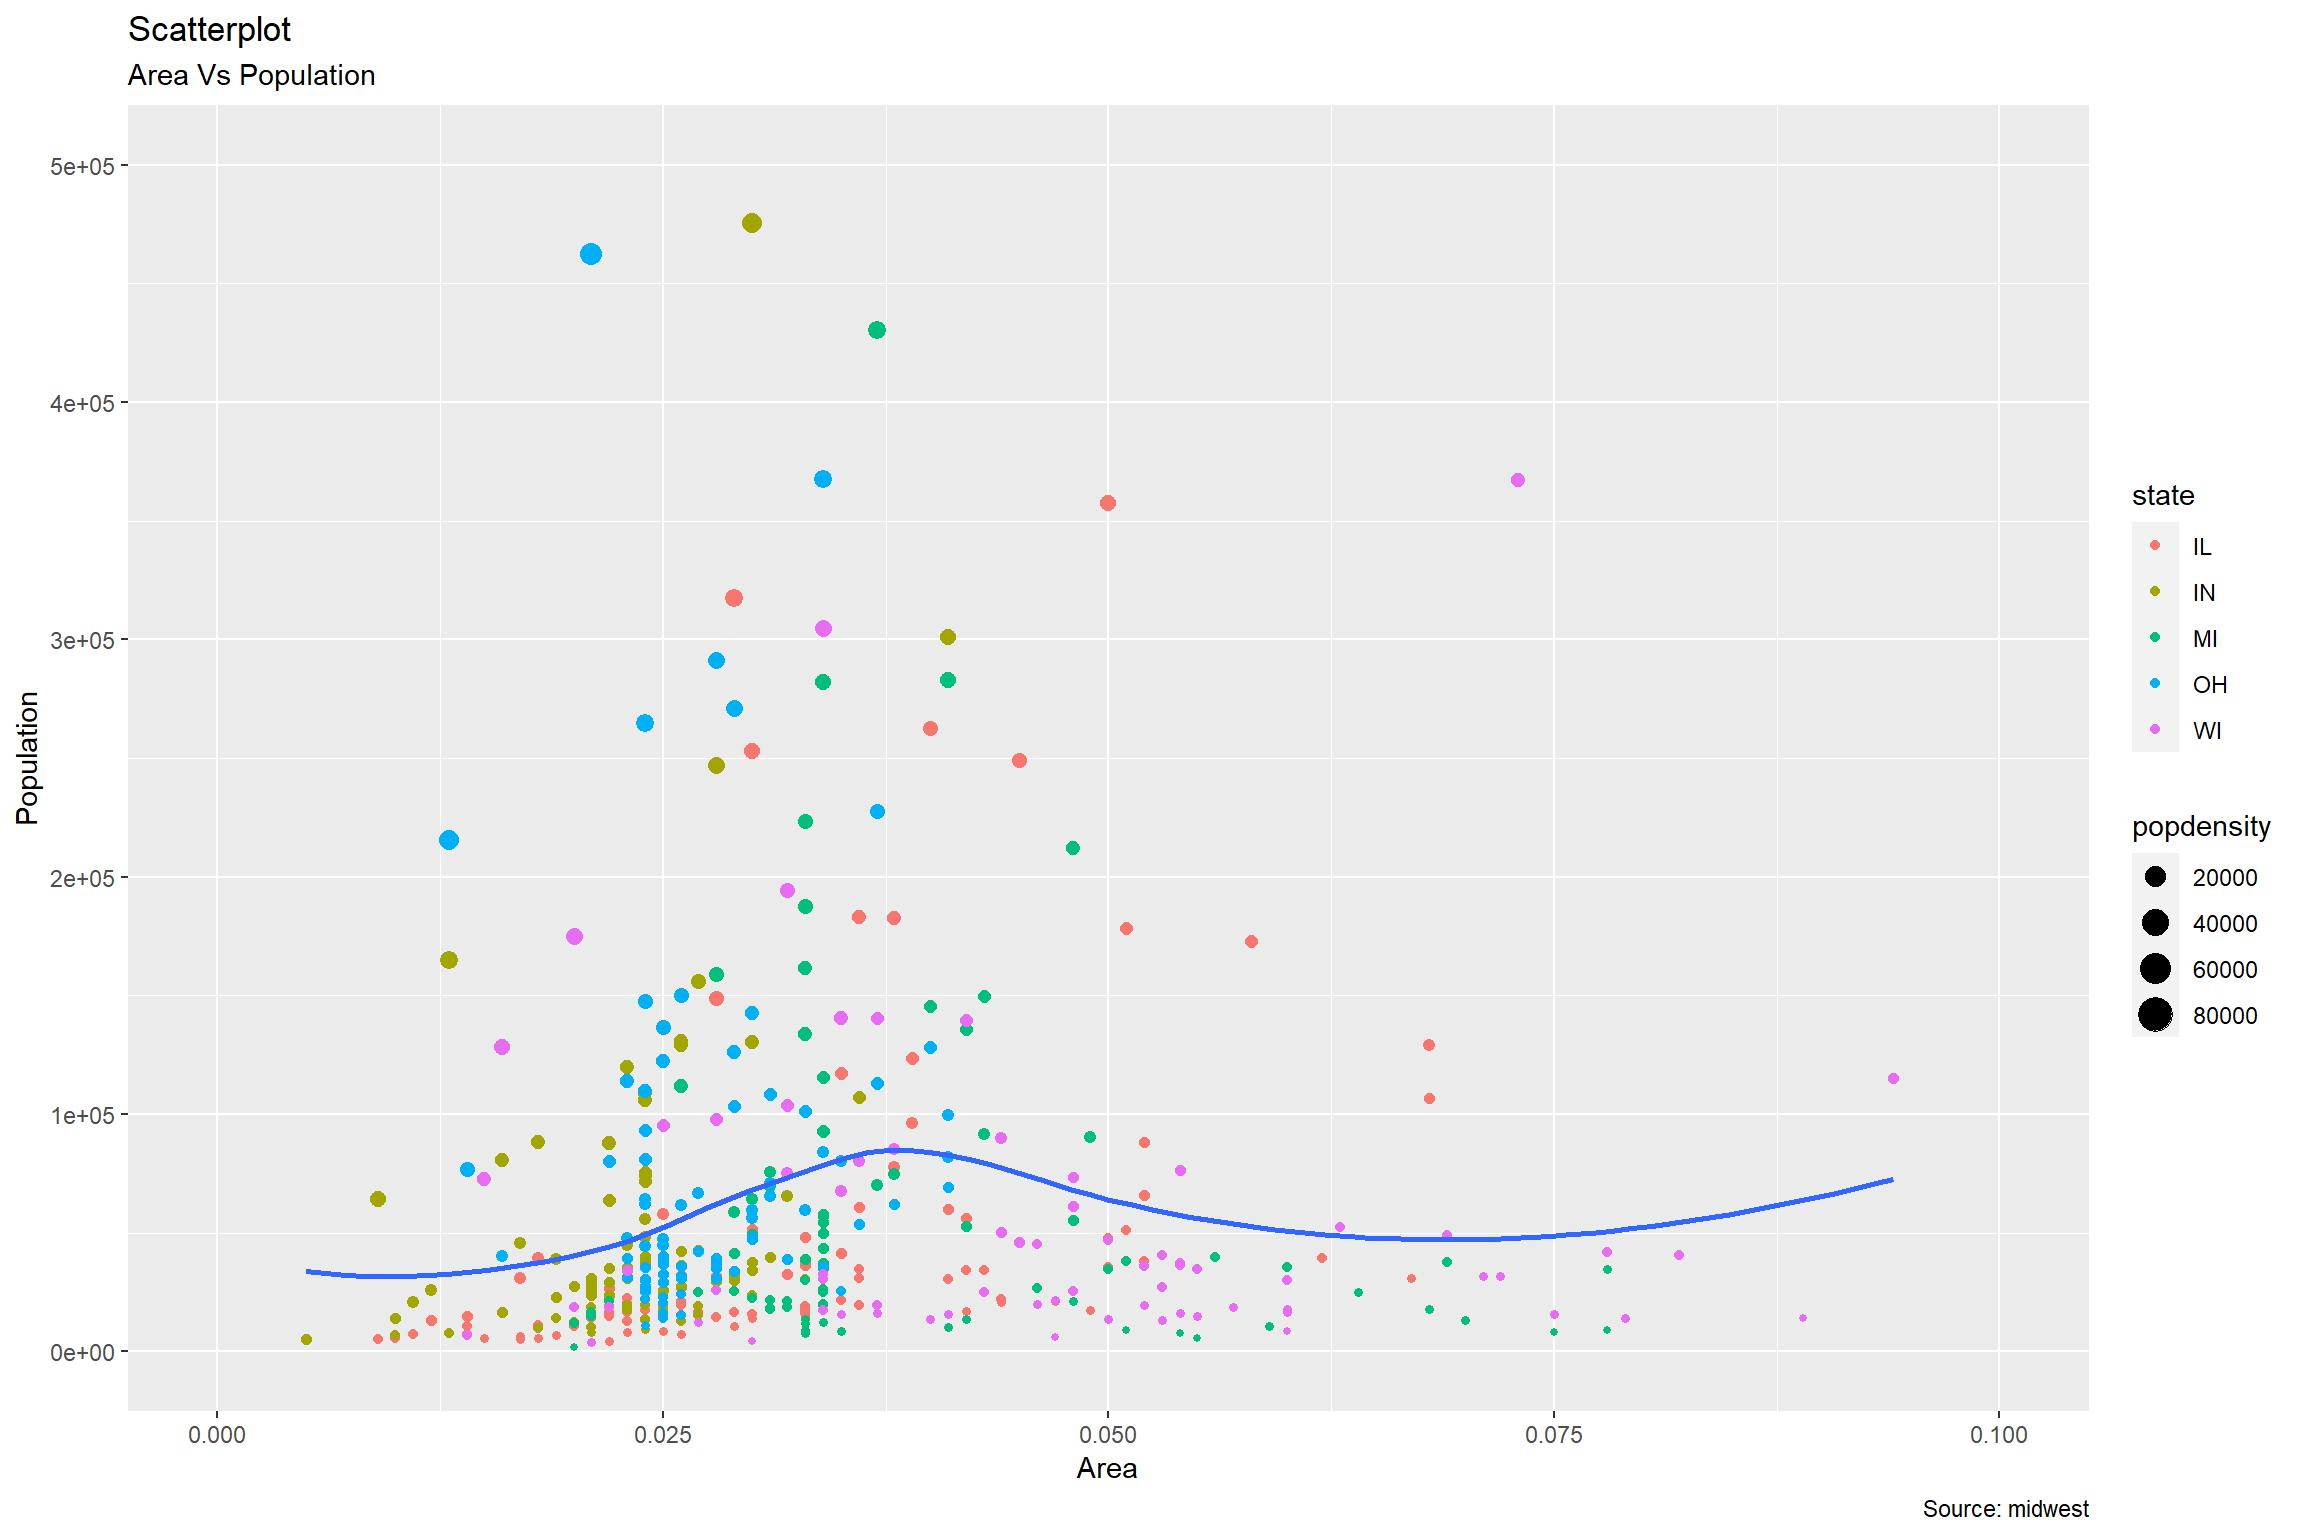
\includegraphics{figures/midwest-1.jpeg}

\begin{Shaded}
\begin{Highlighting}[]
\FunctionTok{plot}\NormalTok{(gg\_themed)}
\end{Highlighting}
\end{Shaded}

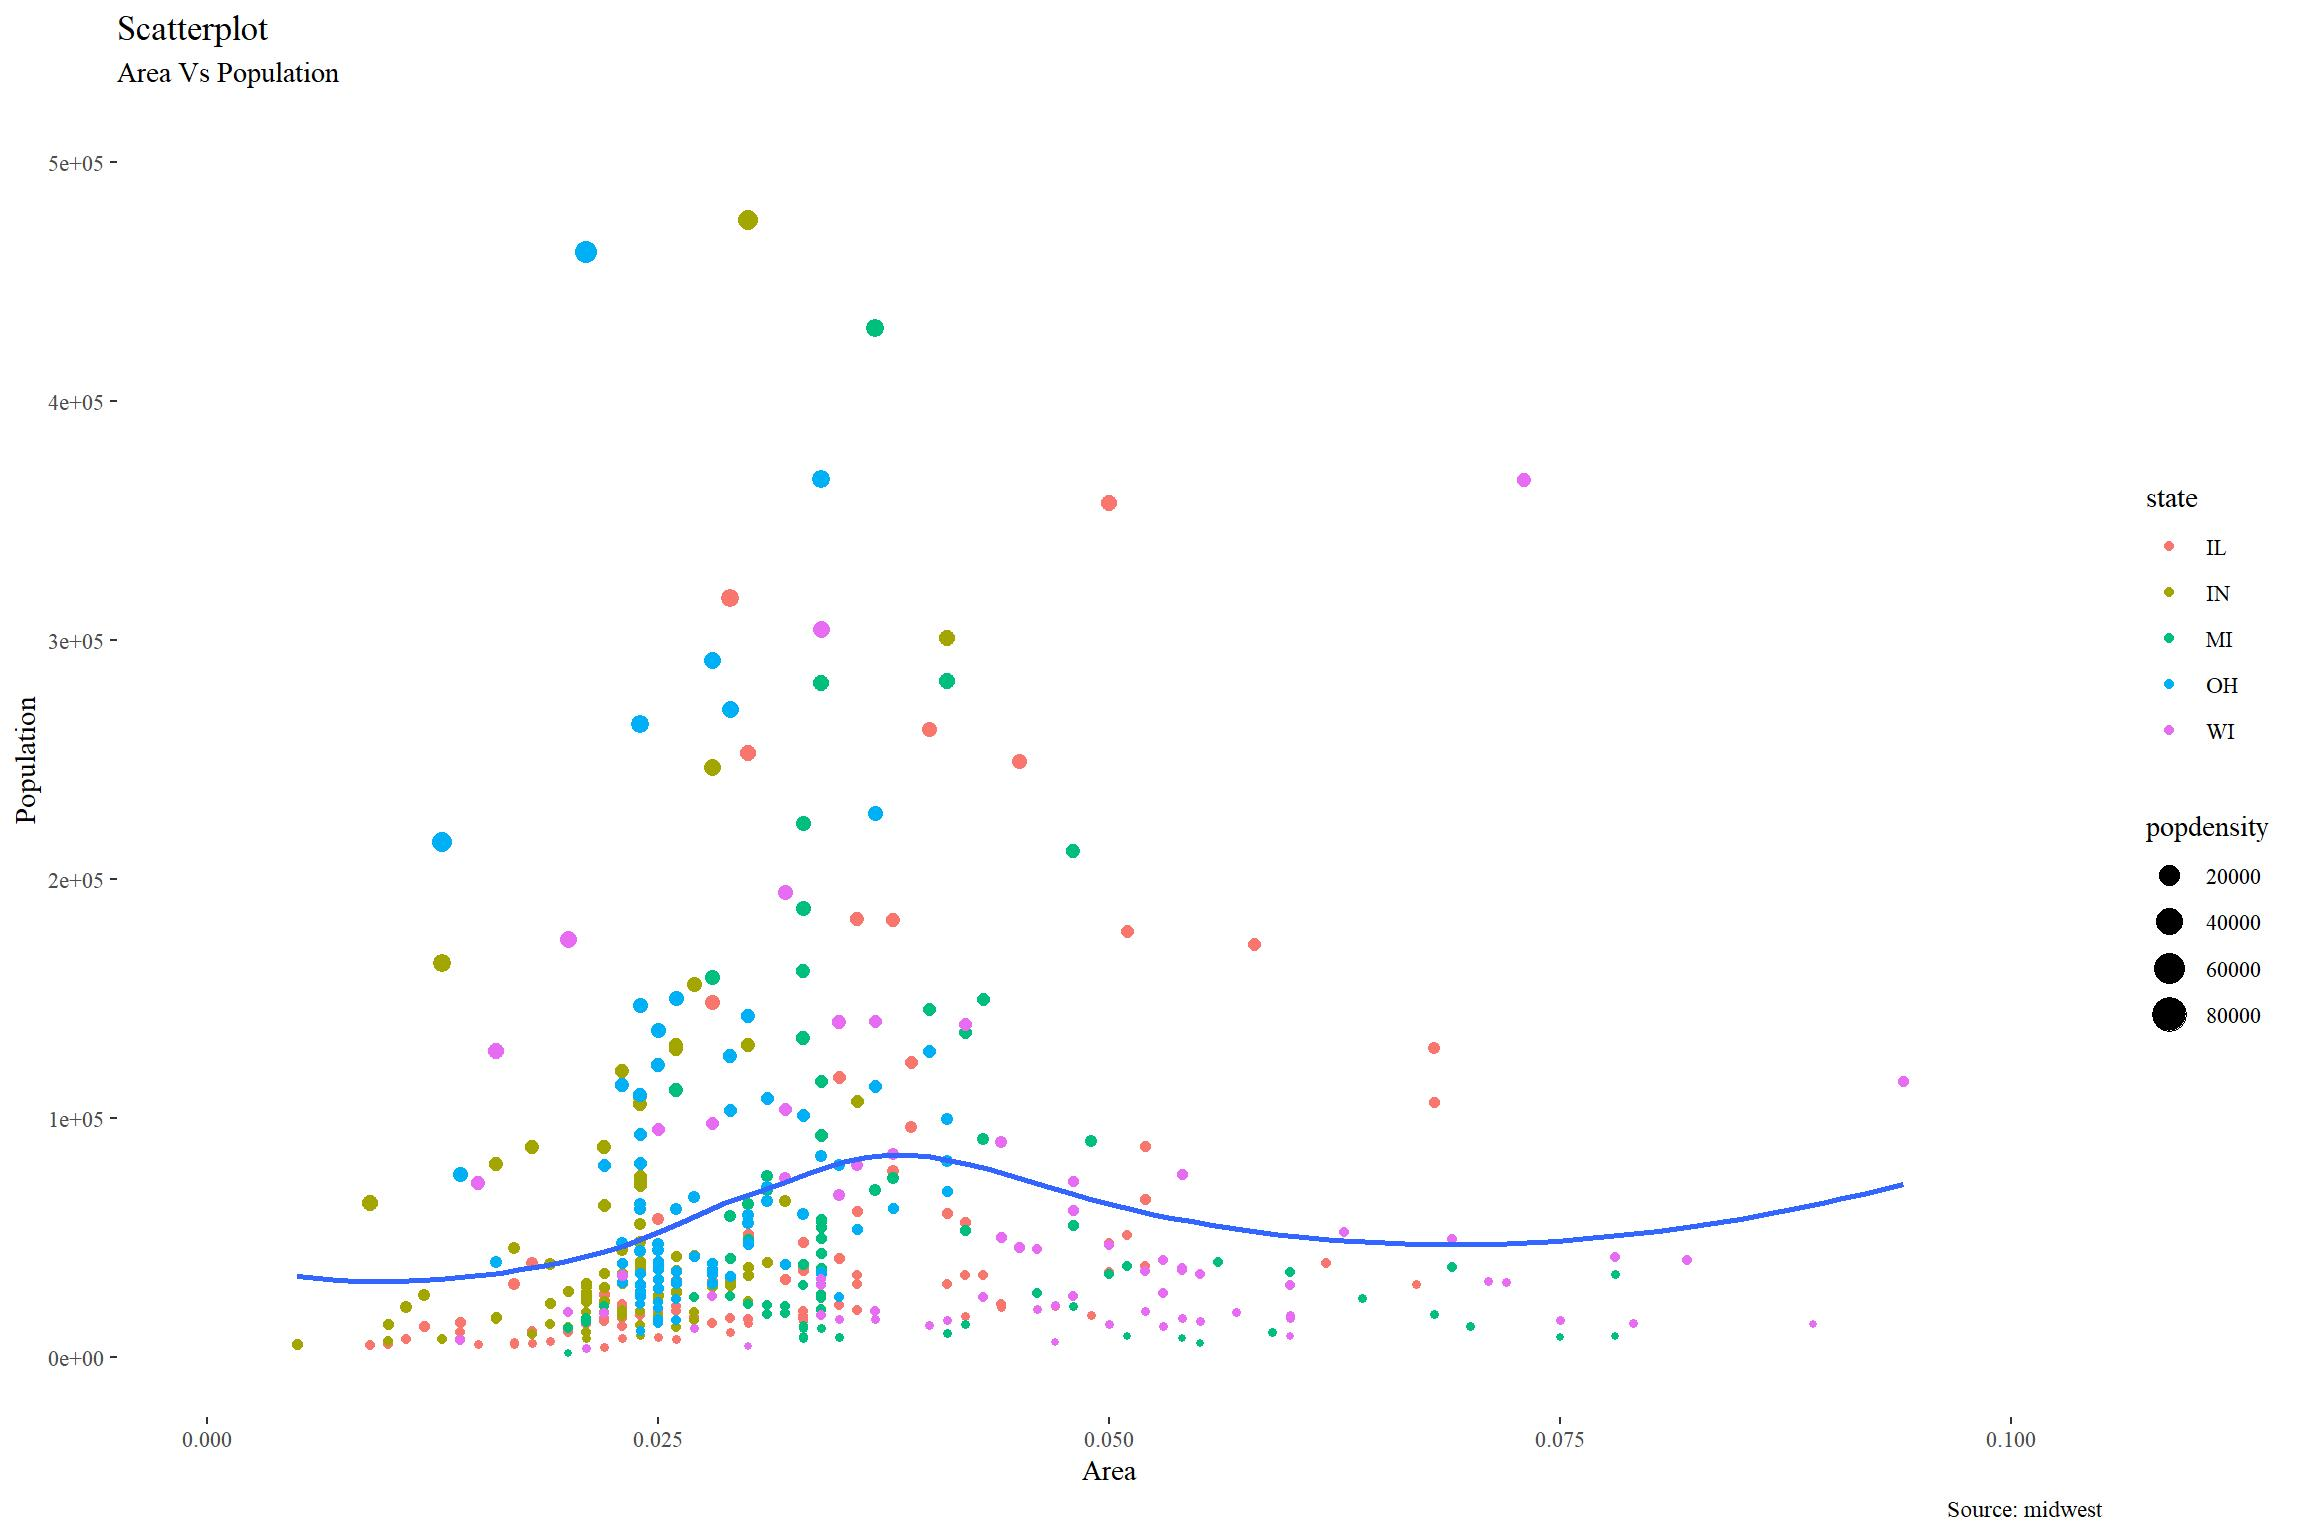
\includegraphics{figures/midwest-2.jpeg}

When you save the notebook, an HTML file containing the code and output
will be saved alongside it (click the \emph{Preview} button or press
\emph{Ctrl+Shift+K} to preview the HTML file).

\hypertarget{some-additional-functionality-with-ggplot-markdown}{%
\section{Some additional functionality with ggplot \&
Markdown}\label{some-additional-functionality-with-ggplot-markdown}}

\hypertarget{can-create-a-variety-of-graphics}{%
\subsubsection{Can create a variety of
graphics}\label{can-create-a-variety-of-graphics}}

Again, this is a great place to leave notes,questions, or explanations
about the figures in the chunk below. We all know we should write better
figure captions or document our thoughts more often before we share a
plot or have to explain it. This is a great place to write while it's
fresh on your mind!

\begin{Shaded}
\begin{Highlighting}[]
\CommentTok{\#specifies when to use scientific notation}
\CommentTok{\#if you want to read more, here\textquotesingle{}s a useful explanation: https://stackoverflow.com/questions/25946047/how{-}to{-}prevent{-}scientific{-}notation{-}in{-}r}
\FunctionTok{options}\NormalTok{(}\AttributeTok{scipen =} \DecValTok{999}\NormalTok{)}
\NormalTok{midwest\_select }\OtherTok{\textless{}{-}}\NormalTok{ midwest[midwest}\SpecialCharTok{$}\NormalTok{poptotal }\SpecialCharTok{\textgreater{}} \DecValTok{350000} \SpecialCharTok{\&} \CommentTok{\#creating catagories for the data}
\NormalTok{                            midwest}\SpecialCharTok{$}\NormalTok{poptotal }\SpecialCharTok{\textless{}=} \DecValTok{500000} \SpecialCharTok{\&} 
\NormalTok{                            midwest}\SpecialCharTok{$}\NormalTok{area }\SpecialCharTok{\textgreater{}} \FloatTok{0.01} \SpecialCharTok{\&} 
\NormalTok{                            midwest}\SpecialCharTok{$}\NormalTok{area }\SpecialCharTok{\textless{}} \FloatTok{0.1}\NormalTok{, ]}

\CommentTok{\# Plot}
\FunctionTok{ggplot}\NormalTok{(midwest, }\FunctionTok{aes}\NormalTok{(}\AttributeTok{x=}\NormalTok{area, }\AttributeTok{y=}\NormalTok{poptotal)) }\SpecialCharTok{+} 
  \FunctionTok{geom\_point}\NormalTok{(}\FunctionTok{aes}\NormalTok{(}\AttributeTok{col=}\NormalTok{state, }\AttributeTok{size=}\NormalTok{popdensity)) }\SpecialCharTok{+}   \CommentTok{\# draw points}
  \FunctionTok{geom\_smooth}\NormalTok{(}\AttributeTok{method=}\StringTok{"loess"}\NormalTok{, }\AttributeTok{se=}\NormalTok{F) }\SpecialCharTok{+} 
  \FunctionTok{xlim}\NormalTok{(}\FunctionTok{c}\NormalTok{(}\DecValTok{0}\NormalTok{, }\FloatTok{0.1}\NormalTok{)) }\SpecialCharTok{+} 
  \FunctionTok{ylim}\NormalTok{(}\FunctionTok{c}\NormalTok{(}\DecValTok{0}\NormalTok{, }\DecValTok{500000}\NormalTok{)) }\SpecialCharTok{+}   \CommentTok{\# draw smoothing line}
  \FunctionTok{geom\_encircle}\NormalTok{(}\FunctionTok{aes}\NormalTok{(}\AttributeTok{x=}\NormalTok{area, }\AttributeTok{y=}\NormalTok{poptotal), }
                \AttributeTok{data=}\NormalTok{midwest\_select, }
                \AttributeTok{color=}\StringTok{"red"}\NormalTok{, }
                \AttributeTok{size=}\DecValTok{2}\NormalTok{, }
                \AttributeTok{expand=}\FloatTok{0.08}\NormalTok{) }\SpecialCharTok{+}   \CommentTok{\# encircle}
  \FunctionTok{labs}\NormalTok{(}\AttributeTok{subtitle=}\StringTok{"Area Vs Population"}\NormalTok{, }
       \AttributeTok{y=}\StringTok{"Population"}\NormalTok{, }
       \AttributeTok{x=}\StringTok{"Area"}\NormalTok{, }
       \AttributeTok{title=}\StringTok{"Scatterplot + Encircle"}\NormalTok{, }
       \AttributeTok{caption=}\StringTok{"Source: midwest"}\NormalTok{)}
\end{Highlighting}
\end{Shaded}

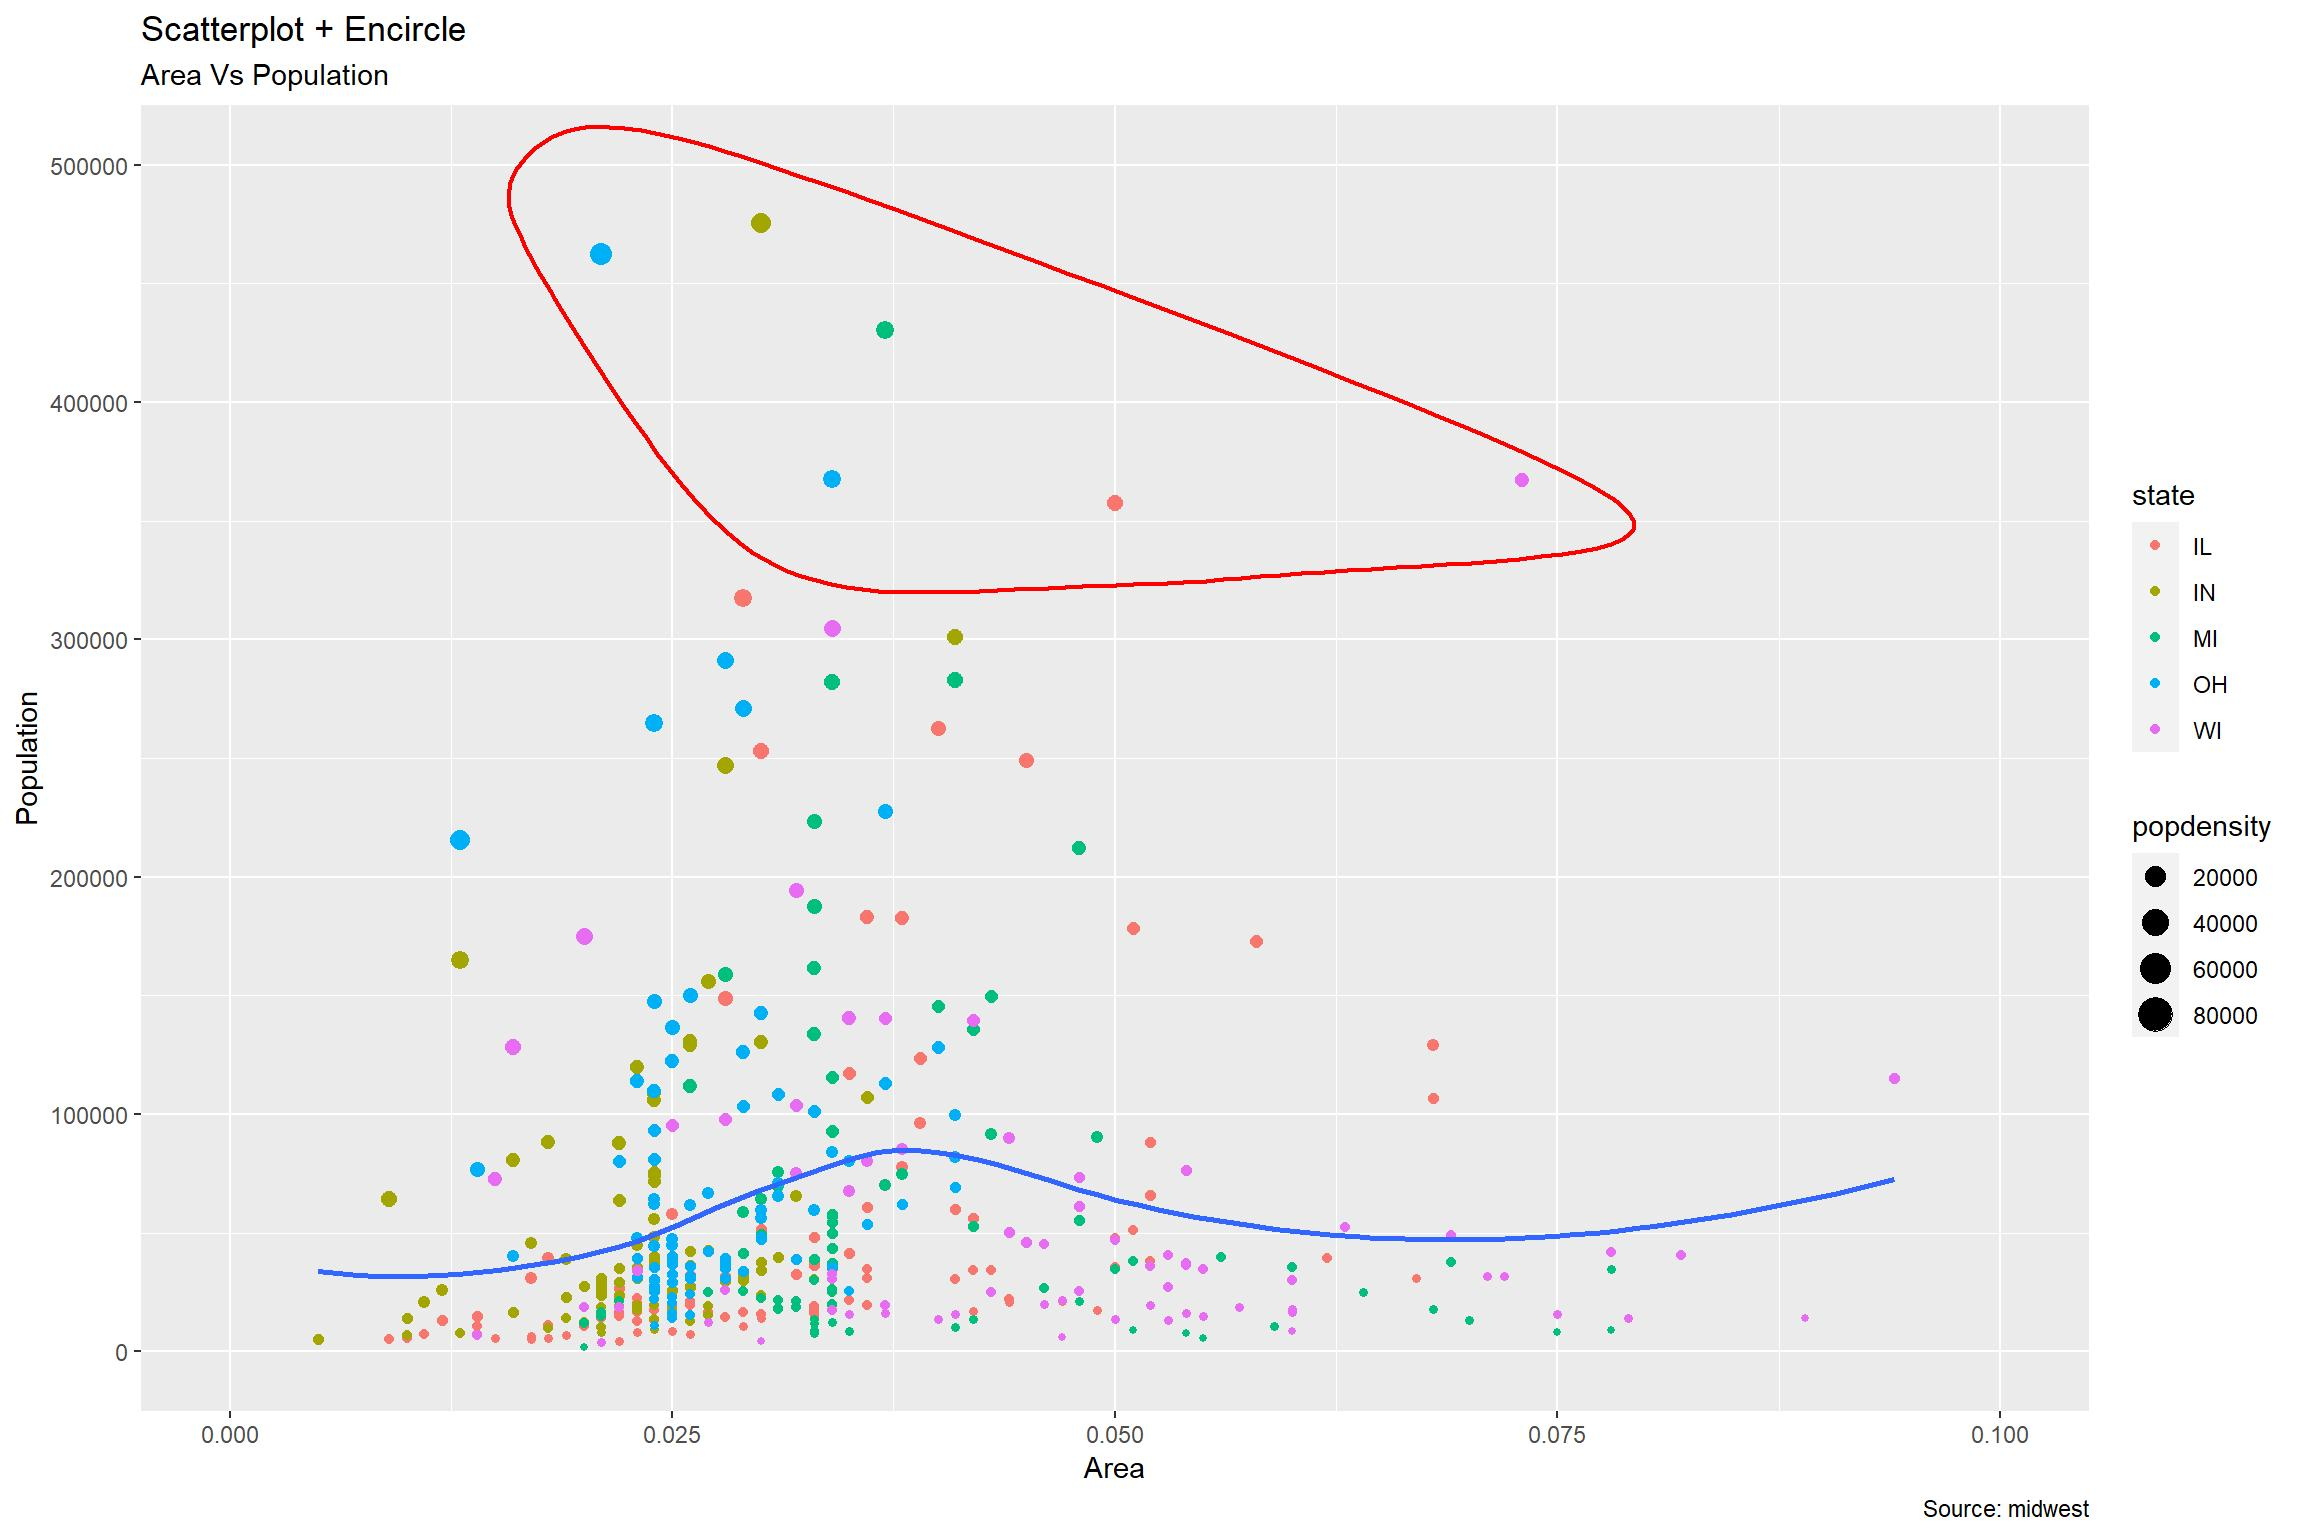
\includegraphics{figures/unnamed-chunk-1-1.jpeg}

\hypertarget{to-prove-ggplot-makes-more-than-scatterplots}{%
\section{To prove ggplot makes more than
scatterplots}\label{to-prove-ggplot-makes-more-than-scatterplots}}

Annotations in an .Rmd do NOT take the place of commenting in line!
Comment. Comment. Comment.

\begin{Shaded}
\begin{Highlighting}[]
\FunctionTok{library}\NormalTok{(ggplot2)}
\FunctionTok{theme\_set}\NormalTok{(}\FunctionTok{theme\_bw}\NormalTok{())  }

\CommentTok{\# Data Prep}
\FunctionTok{data}\NormalTok{(}\StringTok{"mtcars"}\NormalTok{)  }\CommentTok{\# load data}
\NormalTok{mtcars}\SpecialCharTok{$}\StringTok{\textasciigrave{}}\AttributeTok{car name}\StringTok{\textasciigrave{}} \OtherTok{\textless{}{-}} \FunctionTok{rownames}\NormalTok{(mtcars)  }\CommentTok{\# create new column for car names}
\NormalTok{mtcars}\SpecialCharTok{$}\NormalTok{mpg\_z }\OtherTok{\textless{}{-}} \FunctionTok{round}\NormalTok{((mtcars}\SpecialCharTok{$}\NormalTok{mpg }\SpecialCharTok{{-}} \FunctionTok{mean}\NormalTok{(mtcars}\SpecialCharTok{$}\NormalTok{mpg))}\SpecialCharTok{/}\FunctionTok{sd}\NormalTok{(mtcars}\SpecialCharTok{$}\NormalTok{mpg), }\DecValTok{2}\NormalTok{)  }\CommentTok{\# compute normalized mpg}
\NormalTok{mtcars}\SpecialCharTok{$}\NormalTok{mpg\_type }\OtherTok{\textless{}{-}} \FunctionTok{ifelse}\NormalTok{(mtcars}\SpecialCharTok{$}\NormalTok{mpg\_z }\SpecialCharTok{\textless{}} \DecValTok{0}\NormalTok{, }\StringTok{"below"}\NormalTok{, }\StringTok{"above"}\NormalTok{)  }\CommentTok{\# above / below avg flag}
\NormalTok{mtcars }\OtherTok{\textless{}{-}}\NormalTok{ mtcars[}\FunctionTok{order}\NormalTok{(mtcars}\SpecialCharTok{$}\NormalTok{mpg\_z), ]  }\CommentTok{\# sort}
\NormalTok{mtcars}\SpecialCharTok{$}\StringTok{\textasciigrave{}}\AttributeTok{car name}\StringTok{\textasciigrave{}} \OtherTok{\textless{}{-}} \FunctionTok{factor}\NormalTok{(mtcars}\SpecialCharTok{$}\StringTok{\textasciigrave{}}\AttributeTok{car name}\StringTok{\textasciigrave{}}\NormalTok{, }\AttributeTok{levels =}\NormalTok{ mtcars}\SpecialCharTok{$}\StringTok{\textasciigrave{}}\AttributeTok{car name}\StringTok{\textasciigrave{}}\NormalTok{)  }\CommentTok{\# convert to factor to retain sorted order in plot.}

\CommentTok{\# Diverging Barcharts}
\FunctionTok{ggplot}\NormalTok{(mtcars, }\FunctionTok{aes}\NormalTok{(}\AttributeTok{x=}\StringTok{\textasciigrave{}}\AttributeTok{car name}\StringTok{\textasciigrave{}}\NormalTok{, }\AttributeTok{y=}\NormalTok{mpg\_z, }\AttributeTok{label=}\NormalTok{mpg\_z)) }\SpecialCharTok{+} 
  \FunctionTok{geom\_bar}\NormalTok{(}\AttributeTok{stat=}\StringTok{\textquotesingle{}identity\textquotesingle{}}\NormalTok{, }\FunctionTok{aes}\NormalTok{(}\AttributeTok{fill=}\NormalTok{mpg\_type), }\AttributeTok{width=}\NormalTok{.}\DecValTok{5}\NormalTok{)  }\SpecialCharTok{+}
  \FunctionTok{scale\_fill\_manual}\NormalTok{(}\AttributeTok{name=}\StringTok{"Mileage"}\NormalTok{, }
                    \AttributeTok{labels =} \FunctionTok{c}\NormalTok{(}\StringTok{"Above Average"}\NormalTok{, }\StringTok{"Below Average"}\NormalTok{), }
                    \AttributeTok{values =} \FunctionTok{c}\NormalTok{(}\StringTok{"above"}\OtherTok{=}\StringTok{"\#00ba38"}\NormalTok{, }\StringTok{"below"}\OtherTok{=}\StringTok{"\#f8766d"}\NormalTok{)) }\SpecialCharTok{+} 
  \FunctionTok{labs}\NormalTok{(}\AttributeTok{subtitle=}\StringTok{"Normalised mileage from \textquotesingle{}mtcars\textquotesingle{}"}\NormalTok{, }
       \AttributeTok{title=} \StringTok{"Diverging Bars"}\NormalTok{) }\SpecialCharTok{+} 
  \FunctionTok{coord\_flip}\NormalTok{()}
\end{Highlighting}
\end{Shaded}

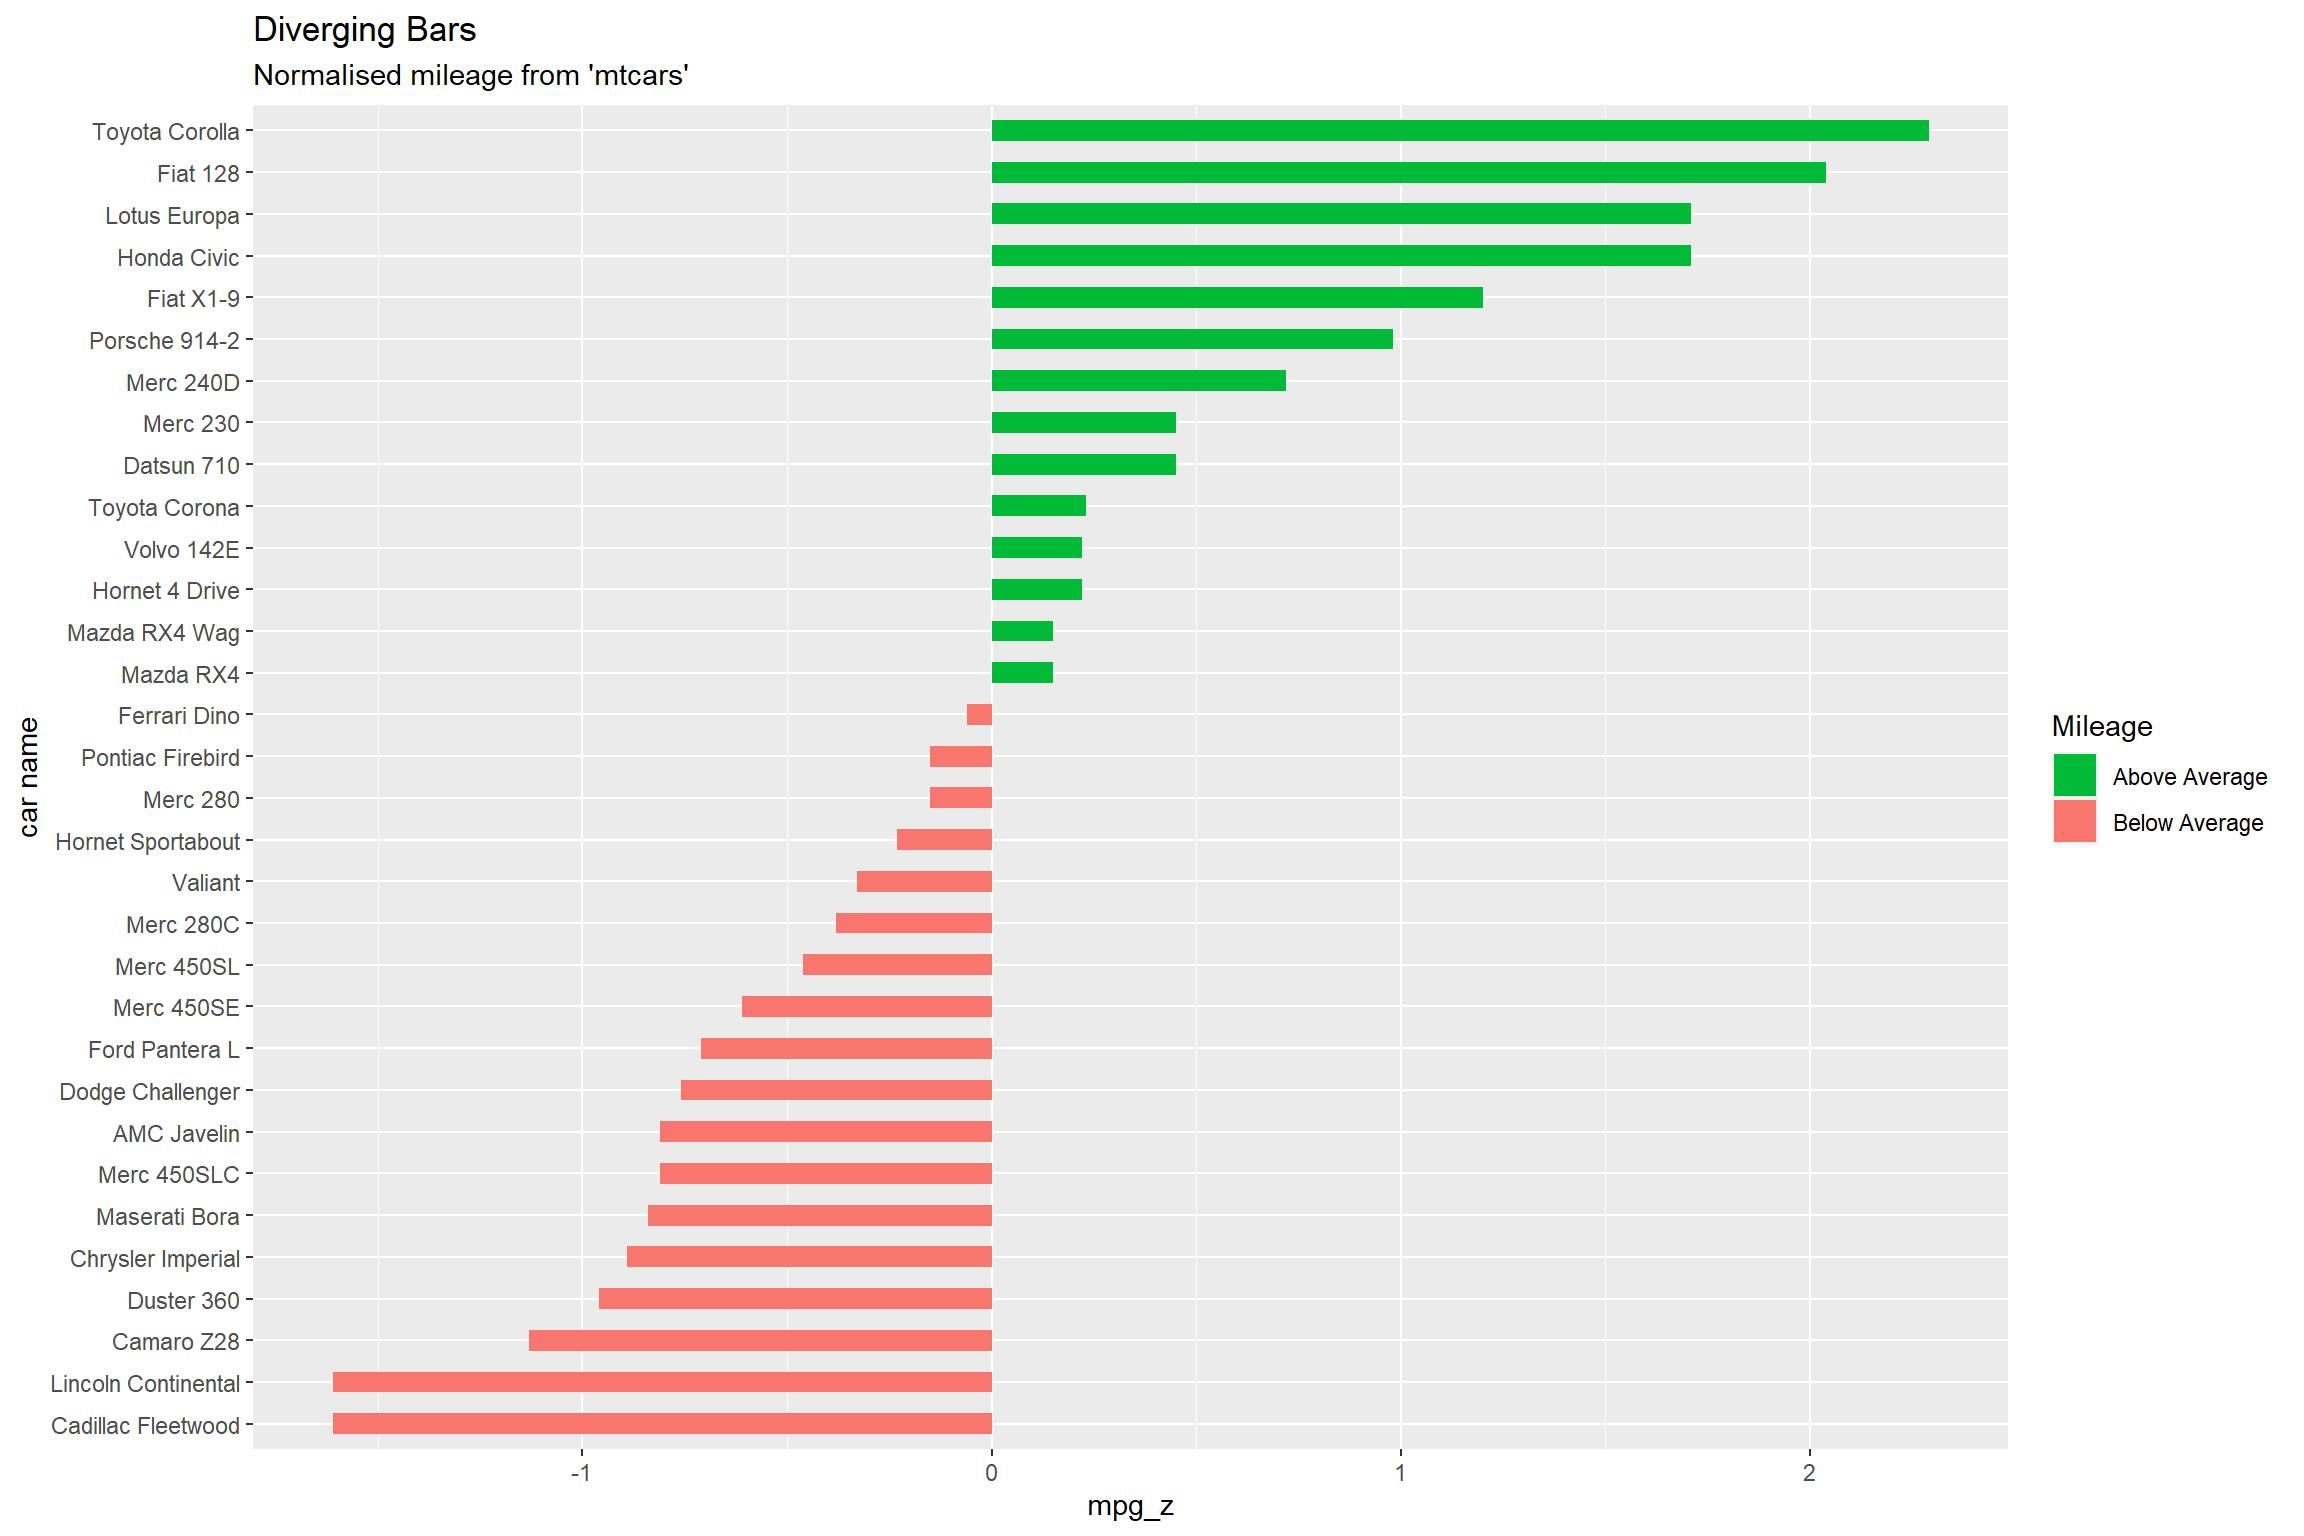
\includegraphics{figures/unnamed-chunk-2-1.jpeg}

\end{document}
